\chapter{Pražská Integrovaná doprava (PID)}
\label{3-teorie-pid}

Pražská integrovaná doprava (PID) je dopravní systém, který zahrnuje jak pozemní
dopravu (tramvaje, železnici, městské a příměstské autobusové linky, lanovou dráhu na Petřín),
tak i tu podzemní (metro). Tento dopravní systém zahrnuje i některé přívozy. 
Systém probíhá integrací společnými přepravními a tarifními podmínkami a jednotným dopravním řešením včetně 
koordinace jízdních řádů. \cite{pid}
\vskip 0.2in
 
\begin{figure}[H] \centering
    
\includegraphics[width=400pt]{./pictures/pid-logo.png}
    \caption[Logo Pražské integrované dopravy]{Logo Pražské integrované dopravy \cite{pid}}
	\label{fig:pid-logo}                                
\end{figure} 

\section{ROPID}

Chod integrace systému zajišťuje Regionální organizátor pražské integrované dopravy (zkráceně ROPID),
což je příspěvková organizace hlavního města Prahy. Jeho úloha je organizační a kontrolní
a ze své práce se odpovídá orgánům samosprávy a státní správy, které jej zabezpečením dopravy pověřily.

\begin{figure}[H] \centering
    
\includegraphics[width=200pt]{./pictures/ropid-logo.jpg}
    \caption[Logo ROPIDu]{Logo ROPIDu \cite{pid}}
	\label{fig:ropid-logo}                                
\end{figure}

ROPID se zabývá vytvářením, rozvíjení, a udržováním systému Pražské integrované dopravy v Praze a okolí,
včetně návazností na jiné systémy jako jsou Integrovaná doprava Plzeňského kraje,
Doprava Ústeckého kraje, Integrovaný dopravní systém Libereckého kraje nebo 
Integrovaná regionální doprava Královéhradeckého a Pardubického kraje.
Taktéž se zabývá vytvářením zásad a standardů dopravní obsluhy a jejich aplikace v závislosti
na dostupných finančních zdrojích a jejich projednání s obcemi, okresními úřady a dopravci.
ROPID výbírá dopravce, uzavírání smluv o závazku veřejné služby jménem města Prahy 
k zajištění provozu PID s dotčenými obcemi, Středočeským krajem a dopravci a kontrola jejich plnění.
Náplní ROPIDu jsou i organizace finančních toků v systému PID, návrh tarifu a jízdného v systému PID a
zajištění jednotnosti informačního systému PID.  \cite{wikipedia-ropid}

\section{Tarifní pásma PID}

\begin{figure}[H] \centering
    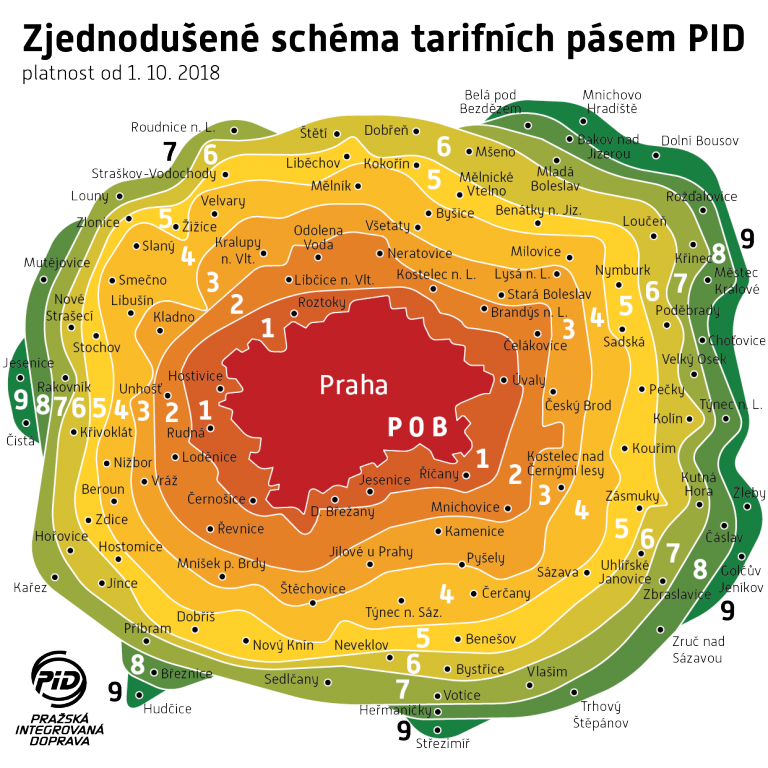
\includegraphics[width=400pt]{./pictures/pasma-schema.png}
    \caption[Schéma tarifních pásem PID]{Schéma tarifních pásem PID \cite{pid}}
	\label{fig:pasma-schema}                                
\end{figure}